%% abtex2-modelo-relatorio-tecnico.tex, v-1.7.1 laurocesar
%% Copyright 2012-2013 by abnTeX2 group at http://abntex2.googlecode.com/ 
%%
%% This work may be distributed and/or modified under the
%% conditions of the LaTeX Project Public License, either version 1.3
%% of this license or (at your option) any later version.
%% The latest version of this license is in
%%   http://www.latex-project.org/lppl.txt
%% and version 1.3 or later is part of all distributions of LaTeX
%% version 2005/12/01 or later.
%%
%% This work has the LPPL maintenance status `maintained'.
%% 
%% The Current Maintainer of this work is the abnTeX2 team, led
%% by Lauro César Araujo. Further information are available on 
%% http://abntex2.googlecode.com/
%%
%% This work consists of the files abntex2-modelo-relatório-tecnico.tex,
%% abntex2-modelo-include-comandos and abntex2-modelo-references.bib
%%

% ------------------------------------------------------------------------
% ------------------------------------------------------------------------
% abnTeX2: Modelo de Relatório Técnico/Acadêmico em conformidade com 
% ABNT NBR 10719:2011 Informação e documentação - Relatório técnico e/ou
% científico - Apresentação
% ------------------------------------------------------------------------ 
% ------------------------------------------------------------------------

\documentclass[
	% -- opções da classe memoir --
	12pt,				% tamanho da fonte
% 	openright,			% capítulos começam em pág ímpar (insere página vazia caso preciso)
	oneside,			% para impressão em verso e anverso. Oposto a oneside
	a4paper,			% tamanho do papel. 
	% -- opções da classe abntex2 --
	%chapter=TITLE,		% títulos de capítulos convertidos em letras maiúsculas
	%section=TITLE,		% títulos de seções convertidos em letras maiúsculas
	%subsection=TITLE,	% títulos de subseções convertidos em letras maiúsculas
	%subsubsection=TITLE,% títulos de subsubseções convertidos em letras maiúsculas
	% -- opções do pacote babel --
	english,			% idioma adicional para hifenização
	french,				% idioma adicional para hifenização
	spanish,			% idioma adicional para hifenização
	brazil,				% o último idioma é o principal do documento
	]{abntex2}


% ---
% PACOTES
% ---
% Pacotes fundamentais 
% ---
\usepackage{cmap}				% Mapear caracteres especiais no PDF
\usepackage{lmodern}			% Usa a fonte Latin Modern
\usepackage[T1]{fontenc}		% Selecao de codigos de fonte.
\usepackage[utf8]{inputenc}		% Codificacao do documento (conversão automática dos acentos)
\usepackage{indentfirst}		% Indenta o primeiro parágrafo de cada seção.
\usepackage{color}				% Controle das cores
\usepackage{graphicx}			% Inclusão de gráficos
\usepackage{booktabs, multicol, multirow, hhline} % Esses includes fazem tabelas bem formatadas
\usepackage[table]{xcolor}
\usepackage{listings}
\usepackage{enumitem}
\usepackage{float}
\usepackage{longtable}

\lstset{
    language=bash, %% Troque para PHP, C, Java, etc... bash é o padrão
    basicstyle=\ttfamily\small,
    numberstyle=\footnotesize,
    % numbers=left,
    % backgroundcolor=\color{gray!10},
    frame=single,
    tabsize=1,
    % rulecolor=\color{black!30},
    title=\lstname,
    escapeinside={\%*}{*)},
    breaklines=true,
    breakatwhitespace=true,
    framextopmargin=1pt,
    framexbottommargin=1pt,
    inputencoding=utf8,
    extendedchars=true,    
    literate={á}{{\'a}}1 {é}{{\'e}}1 {í}{{\'i}}1 {ó}{{\'o}}1 {ú}{{\'u}}1 
              {Á}{{\'A}}1 {É}{{\'E}}1 {Í}{{\'I}}1 {Ó}{{\'O}}1 {Ú}{{\'U}}1
              {à}{{\`a}}1 {è}{{\`e}}1 {ì}{{\`i}}1 {ò}{{\`o}}1 {ù}{{\`u}}1
              {À}{{\`A}}1 {È}{{\'E}}1 {Ì}{{\`I}}1 {Ò}{{\`O}}1 {Ù}{{\`U}}1
              {ä}{{\"a}}1 {ë}{{\"e}}1 {ï}{{\"i}}1 {ö}{{\"o}}1 {ü}{{\"u}}1
              {Ä}{{\"A}}1 {Ë}{{\"E}}1 {Ï}{{\"I}}1 {Ö}{{\"O}}1 {Ü}{{\"U}}1
              {â}{{\^a}}1 {ê}{{\^e}}1 {î}{{\^i}}1 {ô}{{\^o}}1 {û}{{\^u}}1
              {Â}{{\^A}}1 {Ê}{{\^E}}1 {Î}{{\^I}}1 {Ô}{{\^O}}1 {Û}{{\^U}}1
              {œ}{{\oe}}1 {Œ}{{\OE}}1 {æ}{{\ae}}1 {Æ}{{\AE}}1 {ß}{{\ss}}1
              {ű}{{\H{u}}}1 {Ű}{{\H{U}}}1 {ő}{{\H{o}}}1 {Ő}{{\H{O}}}1
              {ç}{{\c c}}1 {Ç}{{\c C}}1 {ø}{{\o}}1 {å}{{\r a}}1 {Å}{{\r A}}1
              {€}{{\euro}}1 {£}{{\pounds}}1 {«}{{\guillemotleft}}1
              {»}{{\guillemotright}}1 {ñ}{{\~n}}1 {Ñ}{{\~N}}1 {¿}{{?`}}1
              {_in}{{$\in$}}1 {_notin}{{$\notin$}}1 {_neq}{{$\neq$}}1
              {_textsubscript}{{\textsubscript{e=(u,v):u$\in$S}}}1
              {_textunderscore_}{{\textunderscore}}1
              {_textsubscript2}{{\textsubscript{e}}}1
}



% ---

% ---
% Pacotes adicionais, usados no anexo do modelo de folha de identificação
% ---
\usepackage{multicol}
\usepackage{multirow}

% ---
% Pacotes de citações
% ---
\usepackage[brazilian,hyperpageref]{backref}	 % Paginas com as citações na bibl
\usepackage[alf]{abntex2cite}	% Citações padrão ABNT

% --- 
% CONFIGURAÇÕES DE PACOTES
% ---
% Configurações do pacote backref
% Usado sem a opção hyperpageref de backref
\renewcommand{\backrefpagesname}{Citado na(s) página(s):~}
% Texto padrão antes do número das páginas
\renewcommand{\backref}{}
% Define os textos da citação
\renewcommand*{\backrefalt}[4]{
	\ifcase #1 %
		Nenhuma citação no texto.%
	\or
		Citado na página #2.%
	\else
		Citado #1 vezes nas páginas #2.%
	\fi}%
% ---

% ---
% Informações de dados para CAPA e FOLHA DE ROSTO
% ---
\titulo{Problema da Mochila Fracionária e Multiplicação de Polinômios}
\autor{Alexandre Marangoni Costa \\ %author1
        André Luiz de Brandão Damasceno \\ %author2
        Antonio José Grandson Busson \\ %author3 
        Beatriz Marques Santiago%author4
    }

\local{Rio de Janeiro - RJ}
\data{2017}
\instituicao{%
  Pontíficia Universidade Católica do Rio de Janeiro
  \par
  Programa de Pós-Graduação em Informática}
\tipotrabalho{Relatório técnico}
% O preambulo deve conter o tipo do trabalho, o objetivo, 
% o nome da instituição e a área de concentração 
\preambulo{Relatório técnico apresentado como requisito
parcial para obtenção de aprovação na disciplina
Projeto e Análise de Algoritmos.}
% ---

% ---
% Configurações de aparência do PDF final

% alterando o aspecto da cor azul
\definecolor{blue}{RGB}{41,5,195}

% informações do PDF
\makeatletter
\hypersetup{
     	%pagebackref=true,
		pdftitle={\@title}, 
		pdfauthor={\@author},
    	pdfsubject={\imprimirpreambulo},
	    pdfcreator={LaTeX with abnTeX2},
		pdfkeywords={abnt}{latex}{abntex}{abntex2}{relatório técnico}, 
		colorlinks=true,       		% false: boxed links; true: colored links
    	linkcolor=blue,          	% color of internal links
    	citecolor=blue,        		% color of links to bibliography
    	filecolor=magenta,      		% color of file links
		urlcolor=blue,
		bookmarksdepth=4
}
\makeatother
% --- 

% --- 
% Espaçamentos entre linhas e parágrafos 
% --- 

% O tamanho do parágrafo é dado por:
\setlength{\parindent}{1.3cm}

% Controle do espaçamento entre um parágrafo e outro:
\setlength{\parskip}{0.2cm}  
% tente também \onelineskip

% ---
% compila o indice
% ---
\makeindex
% ---

% ----
% Início do documento
% ----
\begin{document}

% Retira espaço extra obsoleto entre as frases.
\frenchspacing 

% ----------------------------------------------------------
% ELEMENTOS PRÉ-TEXTUAIS
% ----------------------------------------------------------
% \pretextual

% ---
% Capa
% ---
\imprimircapa
% ---
\cleardoublepage
% ---
% Folha de rosto
% (o * indica que haverá a ficha bibliográfica)
% ---
\imprimirfolhaderosto*
% ---
\cleardoublepage
% ---
% Anverso da folha de rosto:
% ---

% ---
% inserir lista de ilustrações
% ---
% \pdfbookmark[0]{\listfigurename}{lof}
% \listoffigures*
% \cleardoublepage
% ---

% ---
% inserir lista de tabelas
% ---
% \pdfbookmark[0]{\listtablename}{lot}
% \listoftables*
% \cleardoublepage
% ---

% ---
% inserir lista de abreviaturas e siglas
% ---
% \begin{siglas}
%   \item[Fig.] Area of the $i^{th}$ component
%   \item[456] Isto é um número
%   \item[123] Isto é outro número
%   \item[lauro cesar] este é o meu nome
% \end{siglas}
% ---

% ---
% inserir lista de símbolos
% ---
% \begin{simbolos}
%   \item[$ \Gamma $] Letra grega Gama
%   \item[$ \Lambda $] Lambda
%   \item[$ \zeta $] Letra grega minúscula zeta
%   \item[$ \in $] Pertence
% \end{simbolos}
% ---

% ---
% inserir o sumario
% ---
\pdfbookmark[0]{\contentsname}{toc}
\tableofcontents*
\cleardoublepage
\include{abntex2-modelo-include-comandos}
% ---


% ----------------------------------------------------------
% ELEMENTOS TEXTUAIS
% ----------------------------------------------------------
\textual

% ----------------------------------------------------------
% Introdução
% ----------------------------------------------------------
\chapter*[Introdução]{Introdução}
\addcontentsline{toc}{chapter}{Introdução}

Este relatório é resultado de um trabalho prático que desenvolveu códigos para a solução de dois problemas clássicos: Problema da Mochila Fracionária e Multiplicação de Polinômios. Além do desenvolvimento de algoritmos que solucionem esses problemas, este trabalho visa realizar uma análise da complexidade e do desempenho das implementações em relação ao tempo de execução.

O problema da mochila fracionária se enquadra numa classe de algoritmos chamados gulosos \cite{manber1989}. As soluções utilizadas para a resolução desse problema utilizam os seguintes métodos: ordenação, mediana das medianas e uma variação da mediana das medianas onde o pivô é o resultado de uma divisão que tem como divisor o número de elementos de um vetor e o dividendo o somatório da razão do valor pelo peso.
%O algoritmo para a solução do primeiro problema se enquadra numa classe de algoritmos chamados gulosos e pode ser entendido como também como um algoritmo em programação dinâmica \cite{manber1989} em sua modalidade não fracionária.

A solução do segundo problema foi feita usando algoritmos que utilizam 3 estratégias diferentes: por multiplicação direta, divisão e conquista (Karatsuba) e por último foi feita a multiplicação por Transformada de Fourier. Vale ressaltar que nos dois últimos, usa-se a técnica da Divisão e Conquista, porém com abordagens distintas. Estudaremos essas abordagens no Capítulo 2.

Este relatório é complementar ao entregue em 24 de junho de 2017. 


\chapter[Mochila Fracionária]{Mochila Fracionária}
% \addcontentsline{toc}{chapter}{Mochila Fracionária}

O problema da mochila consiste em selecionar um subconjunto de itens de forma que o somatório de seus valores seja maximizado sem exceder a capacidade da mochila. Existem variações do problema mochila, nesse trabalho foi abordado a mochila fracionária, onde os itens podem ser divididos para entrar na mochila. Dado essas premissas, o algoritmo que soluciona essa questão tenta determinar quantas porções de cada objeto devem ser adicionadas à mochila. 

A estrutura geral do algoritmo segue uma classe denominada de algoritmo guloso, ou seja, se seleciona o que é melhor no momento, faz-se uma opção ótima para determinado momento e espera-se que essa coleção de opções ótimas alcance o ótimo global. Para provar a corretude do algoritmo, considera-se, sem perda de generalidade que os objetos disponíveis são enumerados em ordem decrescente de valor por unidade de peso:
\[ v_1/w_1 \geq v_2/w_2 \geq ... \geq v_n/w_n \]
Sendo \( X = (x_1, x_2, x_3, ..., x_4) \) uma solução produzida pelo algoritmo. Se todos os \(x_i\) são iguais a 1, a solução é ótima. Caso contrário, seja j o menor índice cujo \(x_j < 1\). Então, \(x_i = 1\) quando i < j, \(x_i = 0\)  quando i > j, e \( \Sigma_{i=1}^nx_iw_i = W\). Logo, \( V(X) = \Sigma_{i=1}^nx_iw_i\).

Agora Considerando \(Y = (y_1, y_2, y_3, ..., y_4)\) como outra solução viável. Então \( \Sigma_{i=1}^ny_iw_i \leq W\) e \( \Sigma_{i=1}^n(x_i - y_i)w_i \geq 0\). Logo com \( V(Y) = \Sigma_{i=1}^ny_iw_i\), temos:
\[ V(X) - V(Y) = \Sigma_{i=1}^n(x_i - y_i)v_i = \Sigma_{i=1}^n(x_i - y_i)w_i{(v_i/w_i)} \]
Quando i < j, \( x_i = 1 \), então \(x_i - y_i\) é positivo ou zero, enquanto \(v_i/w_i \geq v_j/w_j\), já quando i > j, \( x_i = 0\) e então \(x_i - y_i\) é negativo ou zero, enquanto \(v_i/w_i \leq v_j/w_j\). Dessa forma, para todo i = 1,2,3, .., n é verdade que \((x_i - y_i)(v_i/w_i) \leq (x_i - y_i)(v_j/w_j)\). Então pode-se concluir que: 
\[V(X) - V(Y) \leq (v_j/w_j)\Sigma_{i=1}^n(x_i - y_i)w_i \leq 0\]
Dessa forma, prova-se que não existe solução viável que possua valor estritamente maior que o valor V(X) da solução encontrada pelo algoritmo, logo X é uma solução ótima para o problema da mochila fracionária.

Para este trabalho foram implementados 3 algoritmos com estratégias distintas e realizado uma análise das suas complexidades relacionando-as com seus tempos computacionais. A principal diferença nas complexidades das implementações se deve a variação no método de escolha dos elementos a serem colocados na mochila, sendo que em todos são utilizados como critério a razão entre o valor e o peso do item. 

Conforme pode ser visto no código abaixo, em ambas as estratégias foram utilizadas uma mesma estrutura para armazenar o identificador, o valor, o peso e a razão entre valor e peso de cada item.

\begin{lstlisting}[mathescape=true, label=struct]
struct item
{
  unsigned int id;
  int value;
  int weight;    
  float rate; // Razao entre o valor e peso.  
};
\end{lstlisting}

Vale ressaltar também que ambas as estratégias utilizam as mesmas funções de leitura dos itens a serem computados ($loadItems$) e adição dos itens na mochila ($fillKnapsack$). As 3 estratégias de seleção de itens apresentadas no código abaixo são descritas nas próximas seções.

\begin{lstlisting}[mathescape=true, label=heapsort]
void main (FILE *fileIn, int select)
{
    struct item *items = loadItems (fileIn); // Carrega os Itens.
    
    switch (select) // Seleciona a estratégia.
      case 1: // O(nlog n)        
        heapsortRate (items, n);
        break;
    
      case 2: // O(n)
        kesimo (items, 0, n-1, 0);
        break;
    
      case 3: // O(n2)
        pivot (items, 0, n-1, 0);
        break;
    
    knapsack = fillKnapsack (items, W); // Adiciona na mochila.
}
\end{lstlisting}


\section{Mochila Fracionária utilizando Heapsort}

Nesta implementação é utilizado o algoritmo de ordenação Heapsort, que utiliza uma estrutura de heap para armazenar os itens em ordem decrescente de acordo com sua fração ($valor/peso$). Como existem n elementos e todos são adicionados à heap, a complexidade mínima seria $O(n)$, mas ainda é necessário assim que cada elemento é adicionado, reordenar a heap o que, no pior caso, ocorre em $O(logn)$. Como n elementos são adicionados, a complexidade de construção da heap é $O(nlogn)$.

Avaliando os passos explicados acima, este algoritmo apresenta uma complexidade teórica de $O(nlogn)$. Abaixo segue uma simplificação do código utilizado.

\begin{lstlisting}[mathescape=true, label=heapsort]
void heapsortRate (struct item *list, int length)
{
    struct item aux;
    int cunrrentLength = length;

    buildHeap (list, length); // Constroi a heap.
  
    while (cunrrentLength > 1)
    { // Troca a posicao do primeiro elemento com o ultimo.
      aux = list[0]; 
      list[0] = list[cunrrentLength-1];
      list[cunrrentLength-1] = aux;
      cunrrentLength--;
    
      heapify (list, cunrrentLength, 0); // Reorganiza
    }
}
\end{lstlisting}


\section{Mochila Fracionária utilizando Mediana das Medianas}

Esta implementação faz uso do algoritmo do k-ézimo elemento em que a escolha do pivô é baseada no método da mediana das medianas, usando como critério a razão de valor e peso. Conforme pode ser visto no código abaixo, a função $partition$ retorna a posição do pivô resultante do processamento da mediana das medianas e coloca todos elementos maiores que ele a esquerda e menores a direita, não necessariamente ordenados. Todos esses elementos que ficaram a esquerda tem seu peso somado e comparado a capacidade da mochila. Dependendo do resultado dessa comparação, três passos podem ser seguidos:

\begin{enumerate}
    \item Caso o peso seja igual ao valor da mochila, o $partition$ retorna exatamente o valor da mediana das medianas e todos os elementos da esquerda são adicionados à mochila juntamente com o k-ézimo, sendo esta uma condição de parada.
    \item Caso o peso seja maior que a capacidade, mas o peso menos o peso do item retornado pela mediana das medianas seja menor que a capacidade, este elemento é retornado para que se possa calcular sua fração que deve entrar na mochila de acordo com a capacidade restante (no caso anterior ele entrou inteiro), sendo esta uma condição de parada.
    \item Caso o peso seja maior que a capacidade, os valores a direita do $partition$ são desconsiderados e é realizado uma nova mediana das medianas apenas com os valores das razões a esquerda e realizado uma nova soma dos pesos.
    \item Caso o peso seja menor que a capacidade, esse peso é armazenado, é feito uma nova chamada ao kézimo, com novo partition com os valores da razão a direita do partition anterior e a soma dos pesos é acrescentada a soma anterior armazenada.
\end{enumerate}
A nova soma é novamente comparada a capacidade da mochila e essa iteração ocorre até chegar a alguma das duas condições de parada descritas.

\begin{lstlisting}[mathescape=true, label=medianadasmedianas]
void kesimo (struct item *items, int l, int r, int usedWeight)
{
  int m = partition (items, l, r);
  int sum = usedWeight;

  for (int i = l; i <= m; i++)
    sum += items[i].weight;
    
  if (sum == W || m >= numberItems_-1)  
    return m;  
  else if ( (sum > W) && (sum - items[m].weight <= W) )  
    return m;  
  else if (sum > W)
    return kesimo (items, l, m-1, usedWeight);  
  else  
    return kesimo (items, m+1, r, sum);  
}
\end{lstlisting}


Fazendo uma análise de complexidade paralela ao item anterior, podemos substituir a complexidade de se ordenar os itens $O(nlogn)$ pela complexidade do k-ézimo, $O(n)$. Desta forma, a complexidade teórica desta implementação é $O(n)$.  


\section{Mochila Fracionária utilizando Pivô}

Esta última implementação é semelhante a anterior com a diferença que, no lugar da mediana das medianas, o partition se utiliza de um pivô que é calculado da seguinte forma: \[ pivô = \frac{1}{|K|}\sum_{j\in{K}}\frac{v_j}{w_j}\] onde K é o conjunto de itens considerados.

\begin{lstlisting}[mathescape=true, label=pivot]
findPivot (item, int l, int r)
{
  int k = r + 1 - l;
  float pivot = 0;

  for (int i = l; i <= r; i++){
    pivot += items[i].rate;
  }

  return (pivot/k);
}
\end{lstlisting}

É importante destacar também que a função $partitionPivot$, equivalente a $partition$ mostrada na subseção anterior, altera a posição do item mais próximo ao valor calculado pelo $findPivot$, para a última posição a ser considerada como o última item a ser colocada na mochila. Em seguida os itens até a posição j, tem seus pesos somados e verificado se excede o peso da mochila.

\begin{lstlisting}[mathescape=true, label=pivot]
int partitionPivot (struct item *items, int l, int r)
{
  float pivot = findPivot (items, l, r);
  int posPivot = -1;
  int i = l;
  int j = r;
  
  struct item aux;

  while (1)
  {
    for (; items[i].rate >= pivot && i <= r; i++);
    for (; items[j].rate < pivot && j >= l; j--);
    if (i < j)
    {
      if (items[j].rate == pivot)
      {
        posPivot = i;
      }   
      aux = items[i];
      items[i] = items[j];
      items[j] = aux;
    }
    else
    {
      if (posPivot == -1){
        posPivot = l;
        for (int z = l; z <= j; z++)  
        { // Encontra o item com valor mais proximo do pivot
          if(items[posPivot].rate > items[z].rate)
            posPivot = z;
        }
      }
      
      aux = items[posPivot];
      items[posPivot] = items[j];
      items[j] = aux;
      return j;
    }
  }
}
\end{lstlisting}

Para provar que a complexidade de pior caso pode chegar a $O(n^2)$ vamos aplicar este método no conjunto de dados n abaixo e uma mochila de capacidade 200 mil.

\[valor = \{1; 2; 3; 4; 5; 6; 7\}\]
\[peso = \{10.000.000; 100.000; 1.000; 10; 0,1; 0,001; 0,00001\}\]

Para ficar mais fácil o entendimento, considere a tabela \ref{inicio} que será atualizada a cada iteraçao do k-ézimo:

\begin{table}[!ht]
\centering
\begin{tabular}{r|c|c|c|c|c|c|c}
valor & 1 & 2 & 3 & 4 & 5 & 6 & 7 \\
peso & 10000000 & 100.000 & 1.000 & 10 & 0,1 & 0,001 & 0,00001 \\
valor/peso & 0,0000001 & 0,00002 & 0,003 & 0,4 & 50 & 6000 & 700000 \\
\end{tabular}
    \caption{Dados iniciais}
    \label{inicio}
\end{table}

Para esse dados da tabela \ref{inicio}, o primeiro pivot calculado terá valor $100864,3433$ e apenas o último elemento de n terá razão maior que o pivô e poderá entrar na mochila. Como a capacidade da mochila ainda é muito superior, teremos os dados da tabela \ref{iter1} para realizar um novo k-ézimo.

\begin{table}[!ht]
\centering
\begin{tabular}{r|c|c|c|c|c|c}
valor & 1 & 2 & 3 & 4 & 5 & 6 \\
peso & 10000000 & 100.000 & 1.000 & 10 & 0,1 & 0,001 \\
valor/peso & 0,0000001 & 0,00002 & 0,003 & 0,4 & 50 & 6000 \\
\end{tabular}
    \caption{Dados após a primeira iteração do k-ézimo}
    \label{iter1}
\end{table}

O pivô da segunda iteração terá valor $1008,400503$ e, novamente, apenas 1 elemento tem fração superior ao pivô calculado, somando peso 13 na mochila e resultando nos dados da tabela \ref{iter2} para a nova iteração.

\begin{table}[!ht]
\centering
\begin{tabular}{r|c|c|c|c|c}
valor & 1 & 2 & 3 & 4 & 5 \\
peso & 10.000.000 & 100.000 & 1.000 & 10 & 0,1 \\
valor/peso & 0,0000001 & 0,00002 & 0,003 & 0,4 & 50 \\
\end{tabular}
    \caption{Dados após a segunda iteração do k-ézimo}
    \label{iter2}
\end{table}

Se continuarmos até achar exatamente os elementos que cabem na mochila, teremos chamado a rotina do k-ézimo $O(n)$ vezes, como essa rotina tem complexidade $O(n)$, é possível achar um conjunto de itens em que, no pior caso, a execução pode chegar a ter complexidade $O(n^2)$.


\chapter[Multiplicação de Polinômios]{Multiplicação de Polinômios}
% \addcontentsline{toc}{chapter}{Multiplicacao}

Neste trabalho, o problema da multiplicação de polinômios foi atacado com 3 algoritmos diferentes:

\begin{enumerate}
    \item Algoritmo que faz a multiplicação direta dos polinômios de entrada (O($n^2
$)).
    \item  Algoritmo utilizando divisão-e-conquista (O($n^{log\_23}$
)).
    \item  Algoritmo utilizando a DFT e a FFT (Fast Fourier Transform) (O($nlogn$)).
\end{enumerate}

A importância do estudo da multiplicação de polinômios está na sua aplicabilidade em problemas comuns. Por exemplo, a multiplicação de inteiros dos computadores nada mais é do que a multiplicação de polinômios, já que o inteiro vira um polinômio em base 2, no processador.

Um outro exemplo interessante é na área de processamento de sinais digitais. Quando um sinal é colocado num sistema linear, a saída desse sistema é descrita por uma função matemática idêntica a fórmula da multiplicação de polinômios. Assim, multiplicar polinômios mais rapidamente revolucionou a era das telecomunicações. \cite{dasgupta2006}

\section{Multiplicação Direta}

O produto de dois polinômios de grau $d$ é um polinômio de grau $2d$. Seja o polinômio $A(x) = a_0 + a\_1x + a\_2x^2 + ... + a_{d}x^d$ e o polinômio $B(x) = b_0 + b\_1x + b\_2x^2 + ... + b_{d}x^d$ , o produto destes polinômios $C(x) = c_0 + c\_1x + c\_2x^2 + ...  + a_{2d}x^{2d}$  tem os segintes coeficientes:

\[c_k = a_0b_k + a\_1b_{k-1} + ... + a_kb_o = \sum_{i-0}^{k}{a_ib_{k-i}}\]

O seguinte código para iterar entre $A(x)$ e $B(x)$ para calcular $C(x)$:

\begin{lstlisting}[mathescape=true, label=multiplicacao_direta]
int* multiply_trivial(int A[], int B[], int n) {
    int *C = (int *) calloc(2*n + 1, sizeof(int));
    for (int i = 0; i < n + 1; i++)
        for (int j = 0; j < n + 1; j++)
            C[i+j] += A[i] * B[j];
    return C;
}
\end{lstlisting}

Olhando com atenção, o código é uma transcrição da fórmula acima. Cada $C[i+j]$ corresponde ao $c_k$, e é a soma dos produtos entre $A[i]$ e $B[j]$. Observe que $i+j$ é igual ao $k$ da fórmula.

A análise de complexidade é direta: para cada coeficiente de A passamos por todos os coeficientes de B. Como A e B tem $n$ coeficientes, \textbf{a complexidade é $O(n^2)$}.
%inserir a análise da complexidade de acordo com o código implementado

\section{Divisão e Conquista}

A solução por divisão e conquista da multiplicação de polinômios divide cada polinômio em dois (coeficientes pares e coeficientes ímpares) da seguinte forma:
Seja polinômio A de grau d, onde, por simplicidade d é potencia de 2, 

\[A(x) = a_0 + a\_1x^1 + a\_2x^2 + a_3x^3 + ... + a_{d-2}x^{d-2} + a_{d-1}x^{d-1} + a_{d}x^{d}\] 

Ele pode ser representado da seguinte forma:

\[A(x) = (a_0 + a\_2x^2 + ... + a_{d-2}x^{d-2} + a_{d}x^{d}) + (a\_1 + a_3x^2 + ... +  a_{d-2}x^{d-2})x\] 

Aplicando essa representação sucessivamente, reduzimos o problema à multiplicação $(ax+b)\times(cx+d) = acx^2 + (ad + bc)x + bd$. Apesar de parecer que há a necessidade de 4 multiplicações no código, assim como o Algoritmo de Strassen na multiplicação de matrizes consegue diminuir 8 multiplicações para 7, é possível reduzir de 4 para 3 multiplicações se observamos a seguinte igualdade:

\[(ad + bc) = (a + b)(c + d) - ac - bd \]

Com isso, basta apenas multiplicar $a\times{c}$, $b\times{d}$ e $(a+b)\times(c+d)$

Para analisar a complexidade é necessário observar a relação de recorrência. O problema é dividido pela metade, e são executadas 3 chamadas recursivas, desta forma temos:

\[ T(n) = 3T(n/2) + O(n)\]

Aplicando a relação de recorrência $T(n) = aT(n/b) + O(n^d)$, temos $a = 3$, $b=2$ e $d=1$:

\[\frac{a}{b^d}=\frac{3}{2} > 1\]

Portanto:

\[T(n)=O(n^{\log_{b}{a}})=O(n^{\log3})\]

O código abaixo mostra a implementação desta técnica em C. Foram omitidas as declarações de variáveis e alocações dinâmicas, entre outros detalhes, para simplificação da leitura:
\begin{lstlisting}[mathescape=true, label=divisao_conquista]
int* multiply_divide_conquer(int AB[], int CD[], int n)
{
    // Base case
    if (n < 10)
        return multiply_trivial(AB, CD, n);

    // Divide Step
    int half = n / 2;
    for (int i = 0; i < half; i++) {
        a[i] = AB[i];
        c[i] = CD[i];

        b[i] = AB[i+half];
        d[i] = CD[i+half];
    }

    for(int i = 0; i < half; i++) {
        ab[i] = a[i]+b[i];
        cd[i] = c[i]+d[i];
    }

    // Conquer
    int *ac   = multiply_divide_conquer(a,c, half);
    int *bd   = multiply_divide_conquer(b,d, half);
    int *abcd = multiply_divide_conquer(ab, cd, half);

    // Combine
    for (int i = 0; i < n; i++) {
        result[i]        += ac[i];
        result[i+half]   += abcd[i]  - ac[i] - bd[i];
        result[i+2*half] += bd[i];
    }

    return result;
}
\end{lstlisting}

\section{Transformada Rapida de Fourier}

%achei que ficou meio estranho duas citações seguidas sem nenhuma informação sobre elas... "De acordo com (DASGUPTA; PAPADIMITRIOU; VAZIRANI, 2006), a utilizaçãoda Transformada Rápida de Fourier (FFT) (BRIGHAM, 1988) para redução do tempocomputacional na multiplicação de polinômios..."

De acordo com \cite{dasgupta2006}, a utilização da Transformada Rápida de Fourier (FFT)~\cite{brigham1988f} para redução do tempo computacional na multiplicação de polinômios faz uso do fato de que um polinômio de grau d pode ser representado tanto pelos seus coeficientes quanto pelo seu valor em $d+1$ pontos distintos. Desta forma, o polinômio $C$, de grau $2d$, resultante da multiplicação $(A\times{B})$, também pode ser representado pelo seu valor em $2d+1$ pontos distintos.

Para achar o valor de $C$ em qualquer ponto $z$, basta apenas saber o valor de $A(z)$ e $B(z)$ e multiplica-los. Por ultimo, para saber os coeficientes de $C$ é necessário fazer uma interpolação a partir dos valores nos $d+1$ pontos. Apesar de parecer simples, o cálculo do valor de um polinimio grau $d\le{n}$ em apenas 1 ponto tem complexidade $O(n)$, tomando como base a necessidade de se calcular em n pontos, teremos a complexidade de $O(n^2)$. Para tentar reduzir esta complexidade, usamos a FFT para um conjunto particular de pontos (raízes complexas da unidade), em que é possível reaproveitar passos computacionais.  A FFT utiliza a estratégia de dividir e conquistar, empregando os coeficientes de índices par e os coeficientes de índice ímpar de do polinômio A(x) separadamente para definir os dois novos polinômios de limite de grau \(n/2 A^{[0]}(x) \) e \(n/2 A^{[1]}(x) \), onde \(A^{[0]}\) contém todos os coeficientes de índice par e \(A^{[1]}\) os de índice ímpar:

%\footnote{O conceito degree-bound (limite de grau) n, que equivale ao inteiro estritamente maior que o grau do polinômio, neste caso um polinômio com degree-bound n, pode ser representado por n pares ponto-valor ${(x_0,y_0),(x\_1,y\_1),...(x_{n-1},y_{n-1})}$ e a multiplicação de 2 polinômios com degree-bound n, resulta num polinômio de degree-bound 2n-1.}

\[A^{[0]}(x) = a_0 + a\_2x + a_4x^2 + ... + a_{n-2}x^{n/2-1} \]
\[A^{[1]}(x) = a\_1 + a_3x + a_5x^2 + ... + a_{n-1}x^{n/2-1} \]


Pelo lema das divisão em metades, a lista de valores (\( (\omega_n^0)^2, (\omega_n^1)^2, ..., (\omega_n^{n-1})^2 \)) não consiste em n valores distintos, mas somente nas n/2 raízes (n/2)-ésimas complexas da unidade, com cada raiz ocorrendo exatamente duas vezes. Assim, os polinômios \(A^{[0]}\) e \(A^{[1]}\) de limite de grau n/2 são avaliados recursivamente nas n/2 raízes (n/2)-ésimas complexas da unidade. Esses sub-problemas apresentam exatamente a mesma forma do problema original, mas tem metade dos tamanho. Essa decomposição é a base do algoritmo FFT recursivo descrito abaixo:
 
\begin{lstlisting}[numbers=left, mathescape=true, label=dijkstra.pseudo.vetor]
RECURSIVE_FFT(Vector a){
    int n = a.size;
    if(a == 1)
        retorn a;
    float wn = pow(E,(2*PI*I)/n);
    float w = 1; 
    Vector a0 = getEvenCoefficients(a);
    Vector a1 = getOddCoefficients(a);
    Vector y = createVector(n);
    Vector y0 = RECURSIVE_FFT(a0);
    Vector y1 = RECURSIVE_FFT(a1);
    for(k = 0; k < n/2; k++){
        y[k] = y0[k] + w*y1[k];
        y[k + n/2] = y0[k] + w*y1[k];
        w = w*wn;
    }   
return y;
}
\end{lstlisting}


A função RECURSIVE-FFT descrita na listagem acima, funciona da seguinte forma. As linhas 2 e 3 descrevem a base da recursão. Nesse caso, a DFT de um elemento é o próprio elemento (\( y_0 = a_0 \omega\_1^0 = a_0.1 = a_0\)). As linhas 7 e 8 definem os vetores de coeficientes para os vetores que armazenam os polinômios A0 e A1. As linhas 5, 6 e 15 garantem que \(\omega\) será atualizado corretamente, de tal forma que, sempre que as linhas 13 e 14 são executadas o valor de \(\omega\) recebe \(\omega_n^k\). As linhas 10 e 11 executam os \(DFT_{n/2}\) cálculos para k = 0, 1, ..., n/2 -1.

Para determinar o tempo de execução da função, observa-se que, para dividir o polinômio entre os vetores \(A^{[0]}\) e \(A^{[1]}\) é gasto \( \theta(n) \). Em seguida, cada vetor é passado por parâmetro pelas chamadas recursivas. Dessa forma, a recorrência para o tempo de execução é a seguinte:
\[T(n) = 2T(n/2) + \theta(n)\]
Que segundo o teorema mestre é:
\[T(n) = \theta(nLog(n))\]

\chapter{Resultados}
Esta seção apresenta os resultados da execução dos algoritmos descritos na seção anterior. A Sub-seção 3.1 apresenta os resultados para o problema da mochila fracionária. Em seguida, a Sub-seção 3.2 apresenta os resultados para o problema de multiplicação de polinômios.

\section{Mochila Fracionária}

Para realizar os experimentos do Problema da Mochila Fracionária foram utilizados máquinas de mesma configuração com processador Intel Core i7-6700 3,4 GHz x 8, memória de 15,6 GB e sistema operacional ubuntu 16.04 LTS na versão 64 bits. Os algoritmos foram implementados utilizando a linguagem C e compilados através do gcc 5.4.0.
 
\begin{longtable}{|c|r|r|r|r|r|}
\toprule
\multicolumn{5}{|c|}{\cellcolor{gray!25}\textbf{Heapsort - O(nlogn)}}\\
\midrule
\multicolumn{1}{|c|}{\cellcolor{gray!10}Arquivo} & \multicolumn{1}{|c|}{\cellcolor{gray!10}Itens} &  \multicolumn{1}{|c|}{\cellcolor{gray!10}Tempo} &
\multicolumn{1}{|c|}{\cellcolor{gray!10}Complexidade Teórica} &
\multicolumn{1}{|c|}{\cellcolor{gray!10}Razão}\\ \hline
knap\_1000\_1	&	1000	&	0,000158	&	9965,78	&	1,59	 \\ \hline
knap\_2000\_1	&	2000	&	0,000373	&	21931,57	&	1,70	 \\ \hline
knap\_3000\_1	&	3000	&	0,000592	&	34652,24	&	1,71	 \\ \hline
knap\_4000\_1	&	4000	&	0,000821	&	47863,14	&	1,72	 \\ \hline
knap\_5000\_1	&	5000	&	0,001050	&	61438,56	&	1,71	 \\ \hline
knap\_6000\_1	&	6000	&	0,001302	&	75304,48	&	1,73	 \\ \hline
knap\_7000\_1	&	7000	&	0,001562	&	89411,97	&	1,75	 \\ \hline
knap\_8000\_1	&	8000	&	0,001828	&	103726,27	&	1,76	 \\ \hline
knap\_9000\_1	&	9000	&	0,002048	&	118221,38	&	1,73	 \\ \hline
knap\_10000\_1	&	10000	&	0,002303	&	132877,12	&	1,73	 \\ \hline
knap\_11000\_1	&	11000	&	0,002529	&	147677,37	&	1,71	 \\ \hline
knap\_12000\_1	&	12000	&	0,002783	&	162608,96	&	1,71	 \\ \hline
knap\_13000\_1	&	13000	&	0,003048	&	177660,91	&	1,72	 \\ \hline
knap\_14000\_1	&	14000	&	0,003318	&	192823,95	&	1,72	 \\ \hline
knap\_15000\_1	&	15000	&	0,003623	&	208090,12	&	1,74	 \\ \hline
knap\_16000\_1	&	16000	&	0,003922	&	223452,55	&	1,76	 \\ \hline
knap\_17000\_1	&	17000	&	0,004274	&	238905,20	&	1,79	 \\ \hline
knap\_18000\_1	&	18000	&	0,004561	&	254442,77	&	1,79	 \\ \hline
knap\_19000\_1	&	19000	&	0,004840	&	270060,52	&	1,79	 \\ \hline
knap\_20000\_1	&	20000	&	0,005102	&	285754,25	&	1,79	 \\ \hline
knap\_100000\_1	&	100000	&	0,031747	&	1660964,05	&	1,91	 \\ \hline


\end{longtable}
 


\begin{longtable}{|c|r|r|r|r|r|}
\toprule
\multicolumn{5}{|c|}{\cellcolor{gray!25}\textbf{Mediana das Medianas - O(n)}}\\
\midrule
\multicolumn{1}{|c|}{\cellcolor{gray!10}Arquivo} & \multicolumn{1}{|c|}{\cellcolor{gray!10}Itens} &  \multicolumn{1}{|c|}{\cellcolor{gray!10}Tempo} &
\multicolumn{1}{|c|}{\cellcolor{gray!10}Complexidade Teórica} &
\multicolumn{1}{|c|}{\cellcolor{gray!10}Razão}\\ \hline
% \midrule
\hline
knap\_1000\_1	&	1000	&	0,000090	&	1000	&	9,00	 \\ \hline
knap\_2000\_1	&	2000	&	0,000354	&	2000	&	17,70	 \\ \hline
knap\_3000\_1	&	3000	&	0,000359	&	3000	&	11,97	 \\ \hline
knap\_4000\_1	&	4000	&	0,000690	&	4000	&	17,25	 \\ \hline
knap\_5000\_1	&	5000	&	0,000545	&	5000	&	10,90	 \\ \hline
knap\_6000\_1	&	6000	&	0,001120	&	6000	&	18,67	 \\ \hline
knap\_7000\_1	&	7000	&	0,001292	&	7000	&	18,46	 \\ \hline
knap\_8000\_1	&	8000	&	0,000998	&	8000	&	12,48	 \\ \hline
knap\_9000\_1	&	9000	&	0,001312	&	9000	&	14,58	 \\ \hline
knap\_10000\_1	&	10000	&	0,001546	&	10000	&	15,46	 \\ \hline
knap\_11000\_1	&	11000	&	0,001796	&	11000	&	16,33	 \\ \hline
knap\_12000\_1	&	12000	&	0,001392	&	12000	&	11,60	 \\ \hline
knap\_13000\_1	&	13000	&	0,002532	&	13000	&	19,48	 \\ \hline
knap\_14000\_1	&	14000	&	0,002992	&	14000	&	21,37	 \\ \hline
knap\_15000\_1	&	15000	&	 0,003312	&	15000	&	22,08	 \\ \hline
knap\_16000\_1	&	16000	&	0,001616	&	16000	&	10,10	 \\ \hline
knap\_17000\_1	&	17000	&	0,002497	&	17000	&	14,69	 \\ \hline
knap\_18000\_1	&	18000	&	0,002538	&	18000	&	14,10	 \\ \hline
knap\_19000\_1	&	19000	&	0,003918	&	19000	&	20,62	 \\ \hline
knap\_20000\_1	&	20000	&	0,003777	&	20000	&	18,89	 \\ \hline
knap\_100000\_1	&	100000	&	0,013099	&	100000	&	13,10	 \\ \hline
\end{longtable}




\begin{longtable}{|c|r|r|r|r|r|}
\toprule
\multicolumn{5}{|c|}{\cellcolor{gray!25}\textbf{Pivô - O(n\textsuperscript{2})}}\\
\midrule
\multicolumn{1}{|c|}{\cellcolor{gray!10}Arquivo} & \multicolumn{1}{|c|}{\cellcolor{gray!10}Itens} &  \multicolumn{1}{|c|}{\cellcolor{gray!10}Tempo} &
\multicolumn{1}{|c|}{\cellcolor{gray!10}Complexidade Teórica} &
\multicolumn{1}{|c|}{\cellcolor{gray!10}Razão}\\ \hline
% \midrule
\hline
knap\_1000\_1	&	1000	&	0,000035	&	1000000	&	0,35	 \\ \hline
knap\_2000\_1	&	2000	&	0,000083	&	4000000	&	0,21	 \\ \hline
knap\_3000\_1	&	3000	&	0,000129	&	9000000	&	0,14	 \\ \hline
knap\_4000\_1	&	4000	&	0,000181	&	16000000	&	0,11	 \\ \hline
knap\_5000\_1	&	5000	&	0,000223	&	25000000	&	0,09	 \\ \hline
knap\_6000\_1	&	6000	&	0,000270	&	36000000	&	0,08	 \\ \hline
knap\_7000\_1	&	7000	&	0,000315	&	49000000	&	0,06	 \\ \hline
knap\_8000\_1	&	8000	&	0,000364	&	64000000	&	0,06	 \\ \hline
knap\_9000\_1	&	9000	&	0,000410	&	81000000	&	0,05	 \\ \hline
knap\_10000\_1	&	10000	&	0,000455	&	100000000	&	0,05	 \\ \hline
knap\_11000\_1	&	11000	&	0,000509	&	121000000	&	0,04	 \\ \hline
knap\_12000\_1	&	12000	&	0,000555	&	144000000	&	0,04	 \\ \hline
knap\_13000\_1	&	13000	&	0,000599	&	169000000	&	0,04	 \\ \hline
knap\_14000\_1	&	14000	&	0,000633	&	196000000	&	0,03	 \\ \hline
knap\_15000\_1	&	15000	&	0,000693	&	225000000	&	0,03	 \\ \hline
knap\_16000\_1	&	16000	&	0,000725	&	256000000	&	0,03	 \\ \hline
knap\_17000\_1	&	17000	&	0,000788	&	289000000	&	0,03	 \\ \hline
knap\_18000\_1	&	18000	&	0,000814	&	324000000	&	0,03	 \\ \hline
knap\_19000\_1	&	19000	&	0,000872	&	361000000	&	0,02	 \\ \hline
knap\_20000\_1	&	20000	&	0,000912	&	400000000	&	0,02	 \\ \hline
knap\_100000\_1	&	100000	&	0,004544	&	10000000000	&	0,00	 \\ \hline
\end{longtable}


\begin{figure}[H]
 \centering
 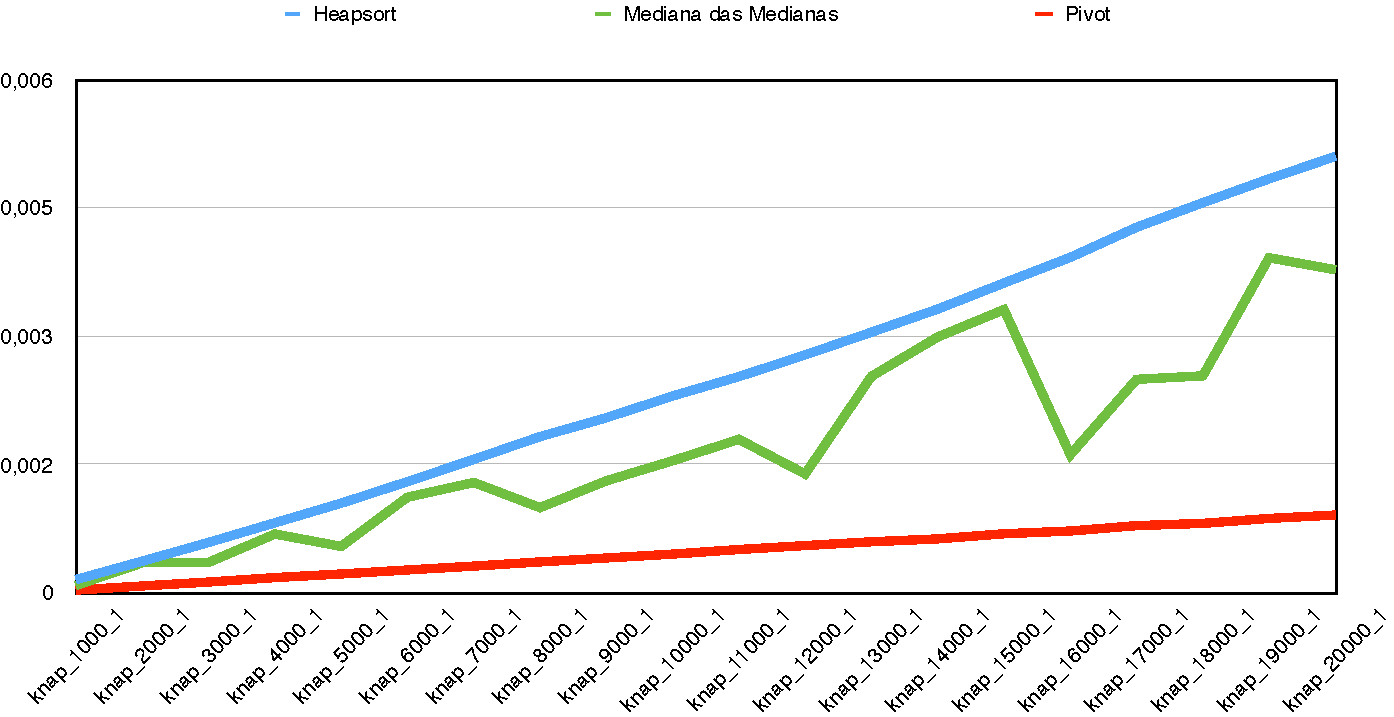
\includegraphics[width=6.4in]{charts/knap_time_1.pdf}
 \caption{Gráfico comparativo entre o TEMPO DE CPU dos algoritmos para o problema da mochila fracionária para as instancias terminadas em \_1}
 \label{fig:AlutGraphTimeAll}
\end{figure}

\begin{figure}[H]
 \centering
 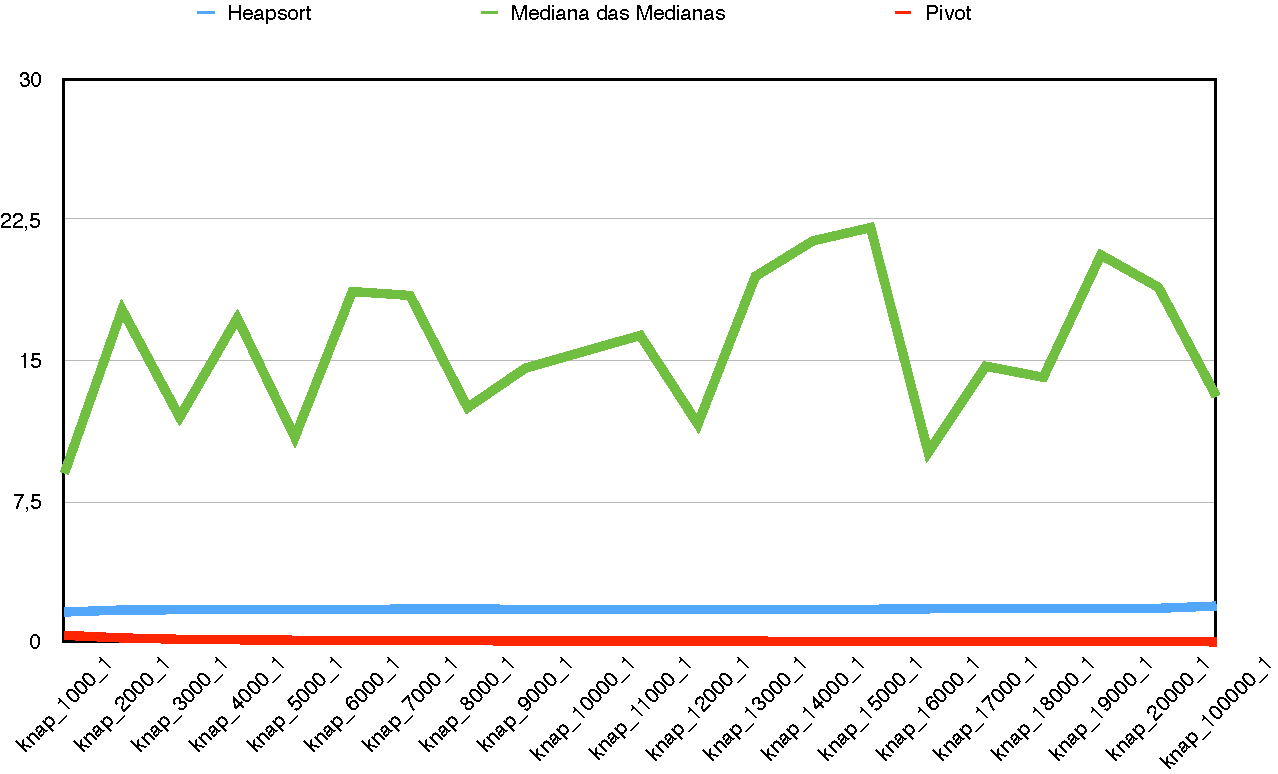
\includegraphics[width=6.4in]{charts/knap_raz_1.pdf}
 \caption{Gráfico comparativo entre a RAZÃO dos algoritmos para o problema da mochila fracionária para as instancias terminadas em \_1}
 \label{fig:AlutGraphTimeAll}
\end{figure}



\begin{longtable}{|c|r|r|r|r|r|}
\toprule
\multicolumn{5}{|c|}{\cellcolor{gray!25}\textbf{Heapsort - O(nlogn)}}\\
\midrule
\multicolumn{1}{|c|}{\cellcolor{gray!10}Arquivo} & \multicolumn{1}{|c|}{\cellcolor{gray!10}Itens} &  \multicolumn{1}{|c|}{\cellcolor{gray!10}Tempo} &
\multicolumn{1}{|c|}{\cellcolor{gray!10}Complexidade Teórica} &
\multicolumn{1}{|c|}{\cellcolor{gray!10}Razão}\\ \hline
knap\_1000\_2	&	1000	&	0,000155	&	9965,78	&	1,56	 \\ \hline
knap\_2000\_2	&	2000	&	0,000373	&	21931,57	&	1,70	 \\ \hline
knap\_3000\_2	&	3000	&	0,000586	&	34652,24	&	1,69	 \\ \hline
knap\_4000\_2	&	4000	&	0,000815	&	47863,14	&	1,70	 \\ \hline
knap\_5000\_2	&	5000	&	0,001059	&	61438,56	&	1,72	 \\ \hline
knap\_6000\_2	&	6000	&	0,001324	&	75304,48	&	1,76	 \\ \hline
knap\_7000\_2	&	7000	&	0,001544	&	89411,97	&	1,73	 \\ \hline
knap\_8000\_2	&	8000	&	0,001819	&	103726,27	&	1,75	 \\ \hline
knap\_9000\_2	&	9000	&	0,002032	&	118221,38	&	1,72	 \\ \hline
knap\_10000\_2	&	10000	&	0,002312	&	132877,12	&	1,74	 \\ \hline
knap\_11000\_2	&	11000	&	0,002574	&	147677,37	&	1,74	 \\ \hline
knap\_12000\_2	&	12000	&	0,002811	&	162608,96	&	1,73	 \\ \hline
knap\_13000\_2	&	13000	&	0,003106	&	177660,91	&	1,75	 \\ \hline
knap\_14000\_2	&	14000	&	0,003307	&	192823,95	&	1,72	 \\ \hline
knap\_15000\_2	&	15000	&	0,003582	&	208090,12	&	1,72	 \\ \hline
knap\_16000\_2	&	16000	&	0,004039	&	223452,55	&	1,81	 \\ \hline
knap\_17000\_2	&	17000	&	0,004216	&	238905,20	&	1,76	 \\ \hline
knap\_18000\_2	&	18000	&	0,004541	&	254442,77	&	1,78	 \\ \hline
knap\_19000\_2	&	19000	&	0,004798	&	270060,52	&	1,78	 \\ \hline
knap\_20000\_2	&	20000	&	0,005084	&	285754,25	&	1,78	 \\ \hline
knap\_100000\_1	&	100000	&	0,031747	&	1660964,05	&	1,91	 \\ \hline
\end{longtable}
 


\begin{longtable}{|c|r|r|r|r|r|}
\toprule
\multicolumn{5}{|c|}{\cellcolor{gray!25}\textbf{Mediana das Medianas - O(n)}}\\
\midrule
\multicolumn{1}{|c|}{\cellcolor{gray!10}Arquivo} & \multicolumn{1}{|c|}{\cellcolor{gray!10}Itens} &  \multicolumn{1}{|c|}{\cellcolor{gray!10}Tempo} &
\multicolumn{1}{|c|}{\cellcolor{gray!10}Complexidade Teórica} &
\multicolumn{1}{|c|}{\cellcolor{gray!10}Razão}\\ \hline
% \midrule
\hline
knap\_1000\_2	&	1000	&	0,000172	&	1000	&	17,20	 \\ \hline
knap\_2000\_2	&	2000	&	0,000422	&	2000	&	21,10	 \\ \hline
knap\_3000\_2	&	3000	&	0,000505	&	3000	&	16,83	 \\ \hline
knap\_4000\_2	&	4000	&	0,000651	&	4000	&	16,28	 \\ \hline
knap\_5000\_2	&	5000	&	0,000749	&	5000	&	14,98	 \\ \hline
knap\_6000\_2	&	6000	&	0,001233	&	6000	&	20,55	 \\ \hline
knap\_7000\_2	&	7000	&	0,001358	&	7000	&	19,40	 \\ \hline
knap\_8000\_2	&	8000	&	0,001772	&	8000	&	22,15	 \\ \hline
knap\_9000\_2	&	9000	&	0,001014	&	9000	&	11,27	 \\ \hline
knap\_10000\_2	&	10000	&	0,001444	&	10000	&	14,44	 \\ \hline
knap\_11000\_2	&	11000	&	0,001177	&	11000	&	10,70	 \\ \hline
knap\_12000\_2	&	12000	&	0,001624	&	12000	&	13,53	 \\ \hline
knap\_13000\_2	&	13000	&	0,001952	&	13000	&	15,02	 \\ \hline
knap\_14000\_2	&	14000	&	0,001393	&	14000	&	9,95	 \\ \hline
knap\_15000\_2	&	15000	&	0,002686	&	15000	&	17,91	 \\ \hline
knap\_16000\_2	&	16000	&	0,002092	&	16000	&	13,08	 \\ \hline
knap\_17000\_2	&	17000	&	0,002272	&	17000	&	13,36	 \\ \hline
knap\_18000\_2	&	18000	&	0,002606	&	18000	&	14,48	 \\ \hline
knap\_19000\_2	&	19000	&	0,002831	&	19000	&	14,90	 \\ \hline
knap\_20000\_2	&	20000	&	0,002901	&	20000	&	14,51	 \\ \hline
knap\_100000\_1	&	100000	&	0,013099	&	100000	&	13,10	 \\ \hline
\end{longtable}


\begin{longtable}{|c|r|r|r|r|r|}
\toprule
\multicolumn{5}{|c|}{\cellcolor{gray!25}\textbf{Pivô - O(n\textsuperscript{2})}}\\
\midrule
\multicolumn{1}{|c|}{\cellcolor{gray!10}Arquivo} & \multicolumn{1}{|c|}{\cellcolor{gray!10}Itens} &  \multicolumn{1}{|c|}{\cellcolor{gray!10}Tempo} &
\multicolumn{1}{|c|}{\cellcolor{gray!10}Complexidade Teórica} &
\multicolumn{1}{|c|}{\cellcolor{gray!10}Razão}\\ \hline
% \midrule
\hline
knap\_1000\_2	&	1000	&	0,000036	&	1000000	&	0,36	 \\ \hline
knap\_2000\_2	&	2000	&	0,000082	&	4000000	&	0,21	 \\ \hline
knap\_3000\_2	&	3000	&	0,000133	&	9000000	&	0,15	 \\ \hline
knap\_4000\_2	&	4000	&	0,000178	&	16000000	&	0,11	 \\ \hline
knap\_5000\_2	&	5000	&	0,000226	&	25000000	&	0,09	 \\ \hline
knap\_6000\_2	&	6000	&	0,000277	&	36000000	&	0,08	 \\ \hline
knap\_7000\_2	&	7000	&	0,000318	&	49000000	&	0,06	 \\ \hline
knap\_8000\_2	&	8000	&	0,000362	&	64000000	&	0,06	 \\ \hline
knap\_9000\_2	&	9000	&	0,000402	&	81000000	&	0,05	 \\ \hline
knap\_10000\_2	&	10000	&	0,000455	&	100000000	&	0,05	 \\ \hline
knap\_11000\_2	&	11000	&	0,000496	&	121000000	&	0,04	 \\ \hline
knap\_12000\_2	&	12000	&	0,000549	&	144000000	&	0,04	 \\ \hline
knap\_13000\_2	&	13000	&	0,000592	&	169000000	&	0,04	 \\ \hline
knap\_14000\_2	&	14000	&	0,000642	&	196000000	&	0,03	 \\ \hline
knap\_15000\_2	&	15000	&	0,000689	&	225000000	&	0,03	 \\ \hline
knap\_16000\_2	&	16000	&	0,000751	&	256000000	&	0,03	 \\ \hline
knap\_17000\_2	&	17000	&	0,000783	&	289000000	&	0,03	 \\ \hline
knap\_18000\_2	&	18000	&	0,000836	&	324000000	&	0,03	 \\ \hline
knap\_19000\_2	&	19000	&	0,000866	&	361000000	&	0,02	 \\ \hline
knap\_20000\_2	&	20000	&	0,000920	&	400000000	&	0,02	 \\ \hline
knap\_100000\_1	&	100000	&	0,004544	&	10000000000	&	0,00	 \\ \hline
\end{longtable}




\begin{figure}[H]
 \centering
 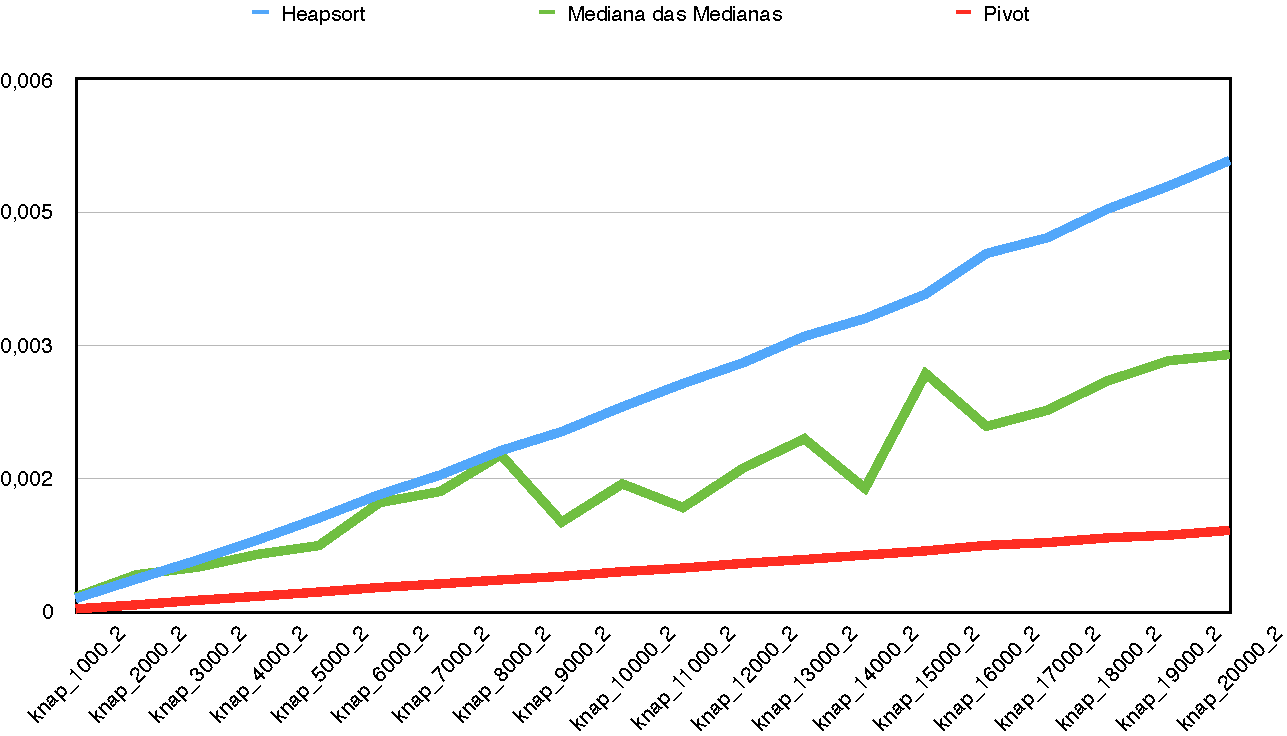
\includegraphics[width=6.4in]{charts/knap_time_2.pdf}
 \caption{Gráfico comparativo entre o TEMPO DE CPU dos algoritmos para o problema da mochila fracionária para as instancias terminadas em \_2.}
 \label{fig:AlutGraphTimeAll}
\end{figure}

\begin{figure}[H]
 \centering
 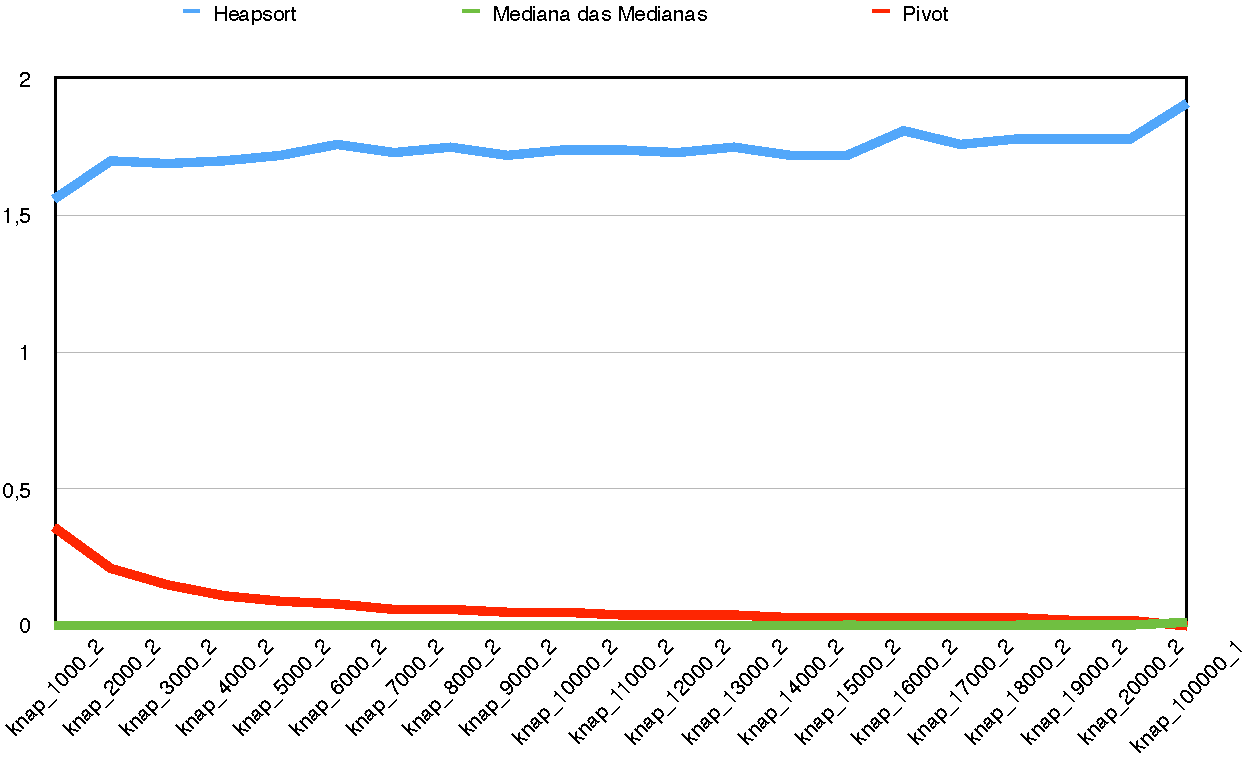
\includegraphics[width=6.4in]{charts/knap_raz_2.pdf}
 \caption{Gráfico comparativo entre a RAZÃO dos algoritmos para o problema da mochila fracionária para as instancias terminadas em \_2.}
 \label{fig:AlutGraphTimeAll}
\end{figure}


\section{Multiplicação de Polinômios}

Para realizar os experimentos do Problema da Multiplicação de Polinômios foram utilizados máquinas de mesma configuração com processador Intel(R) Core(TM) i5-2410M CPU @ 2.30GHz x 4, memória de 8 GB e sistema operacional Manjaro Linux na versão 64 bits. Os algoritmos foram implementados utilizando a linguagem C e compilados através do gcc 6.3.1.

\begin{table}[H]
  \centering    
  \begin{tabular}{|c|r|r|r|r|r|r|r|r|r|}
    \toprule
    \multicolumn{1}{|c|}{\cellcolor{gray!25}\textbf{}} &
    \multicolumn{3}{|c|}{\cellcolor{gray!25}\textbf{Trivial}} \\
    \midrule
    \multicolumn{1}{|c|}{\cellcolor{gray!10}n} &
    \multicolumn{1}{|c|}{\cellcolor{gray!10}Tempo} &
    \multicolumn{1}{|c|}{\cellcolor{gray!10}$n^2$} &
    \multicolumn{1}{|c|}{\cellcolor{gray!10}Razão} \\
    4	&	0,0000003	&	16	&	1,73	 \\ \hline
    8	&	0,0000006	&	64	&	0,89	 \\ \hline
    16	&	0,0000022	&	256	&	0,85	 \\ \hline
    32	&	0,0000110	&	1024	&	1,07	 \\ \hline
    64	&	0,0000243	&	4096	&	0,59	 \\ \hline
    128	&	0,0000860	&	16384	&	0,52	 \\ \hline
    256	&	0,0003600	&	65536	&	0,55	 \\ \hline
    512	&	0,0012800	&	262144	&	0,49	 \\ \hline
    1024	&	0,0047467	&	1048576	&	0,45	 \\ \hline
    2048	&	0,0189000	&	4194304	&	0,45	 \\ \hline
    4096	&	0,0760000	&	16777216	&	0,45	 \\ \hline
    8192	&	0,3053333	&	67108864	&	0,45	 \\ \hline
    16384	&	1,2299999	&	268435456	&	0,46	 \\ \hline
    32768	&	4,8496662	&	1073741824	&	0,45	 \\ \hline
    65536	&	19,4083315	&	4294967296	&	0,45	 \\ \hline
    131072	&	78,4116590	&	17179869184	&	0,46	 \\ \hline
    262144	&	317,4866350	&	68719476736	&	0,46	 \\ \hline
    524288	&	1521,8165150	&	274877906944	&	0,55	 \\ \hline
    1048576	&	5113,8961550	&	1099511627776	&	0,47	 \\ \hline

  \end{tabular}
  \caption{Tabela de resultados da Multiplicação de Polinômios para a solução Trivial. O cálculo da razão foi feito dividindo o tempo pela complexidade. As razões foram multiplicadas por uma constante para facilitar a leitura (entre $10^0$ e $10^3$)}  
  \label{tab:polymul}
\end{table}

\begin{table}[H]
  \centering    
  \begin{tabular}{|c|r|r|r|r|r|r|r|r|r|}
    \toprule
    \multicolumn{1}{|c|}{\cellcolor{gray!25}\textbf{}} &
    \multicolumn{3}{|c|}{\cellcolor{gray!25}\textbf{Karatsuba}} \\
    \midrule
    \multicolumn{1}{|c|}{\cellcolor{gray!10}n} &
    \multicolumn{1}{|c|}{\cellcolor{gray!10}Tempo} &
    \multicolumn{1}{|c|}{\cellcolor{gray!10}$n^{\log_{2}{3}}$} &
    \multicolumn{1}{|c|}{\cellcolor{gray!10}Razão} \\
    4	&	0,0000003	&	9	&	3,11	 \\ \hline
    8	&	0,0000005	&	27	&	1,94	 \\ \hline
    16	&	0,0000023	&	81	&	2,80	 \\ \hline
    32	&	0,0000093	&	243	&	3,84	 \\ \hline
    64	&	0,0000257	&	729	&	3,52	 \\ \hline
    128	&	0,0000810	&	2187	&	3,70	 \\ \hline
    256	&	0,0002400	&	6561	&	3,66	 \\ \hline
    512	&	0,0007467	&	19683	&	3,79	 \\ \hline
    1024	&	0,0022400	&	59049	&	3,79	 \\ \hline
    2048	&	0,0065333	&	177147	&	3,69	 \\ \hline
    4096	&	0,0210333	&	531441	&	3,96	 \\ \hline
    8192	&	0,0593333	&	1594323	&	3,72	 \\ \hline
    16384	&	0,1843333	&	4782969	&	3,85	 \\ \hline
    32768	&	0,5916666	&	14348907	&	4,12	 \\ \hline
    65536	&	1,6649995	&	43046721	&	3,87	 \\ \hline
    131072	&	4,9699995	&	129140163	&	3,85	 \\ \hline
    262144	&	15,2566650	&	387420489	&	3,94	 \\ \hline
    524288	&	44,7499950	&	1162261467	&	3,85	 \\ \hline
    1048576	&	134,1533200	&	3486784401	&	3,85	 \\ \hline
  \end{tabular}
  \caption{Tabela de resultados da Multiplicação de Polinômios para a solução Karatsuba. O cálculo da razão foi feito dividindo o tempo pela complexidade. As razões foram multiplicadas por uma constante para facilitar a leitura (entre $10^0$ e $10^3$)}  
  \label{tab:polymul}
\end{table}

\begin{table}[H]
  \centering    
  \begin{tabular}{|c|r|r|r|r|r|r|r|r|r|}
    \toprule
    \multicolumn{1}{|c|}{\cellcolor{gray!25}\textbf{}} &
    \multicolumn{3}{|c|}{\cellcolor{gray!25}\textbf{Fourier}} \\
    \midrule
    \multicolumn{1}{|c|}{\cellcolor{gray!10}n} &
    \multicolumn{1}{|c|}{\cellcolor{gray!10}Tempo} &
    \multicolumn{1}{|c|}{\cellcolor{gray!10}$n\log{n}$} &
    \multicolumn{1}{|c|}{\cellcolor{gray!10}Razão} \\
    4	&	0,00003	&	8	&	380,54	 \\ \hline
    8	&	0,00006	&	24	&	263,96	 \\ \hline
    16	&	0,00014	&	64	&	212,81	 \\ \hline
    32	&	0,00028	&	160	&	176,87	 \\ \hline
    64	&	0,00061	&	384	&	158,33	 \\ \hline
    128	&	0,00128	&	896	&	143,34	 \\ \hline
    256	&	0,00262	&	2048	&	127,93	 \\ \hline
    512	&	0,00537	&	4608	&	116,46	 \\ \hline
    1024	&	0,01116	&	10240	&	108,98	 \\ \hline
    2048	&	0,02250	&	22528	&	99,88	 \\ \hline
    4096	&	0,04803	&	49152	&	97,72	 \\ \hline
    8192	&	0,09933	&	106496	&	93,27	 \\ \hline
    16384	&	0,20667	&	229376	&	90,10	 \\ \hline
    32768	&	0,42033	&	491520	&	85,52	 \\ \hline
    65536	&	0,86833	&	1048576	&	82,81	 \\ \hline
    131072	&	1,76833	&	2228224	&	79,36	 \\ \hline
    262144	&	3,78667	&	4718592	&	80,25	 \\ \hline
    524288	&	7,56000	&	9961472	&	75,89	 \\ \hline
    1048576	&	15,46000	&	20971520	&	73,72	 \\ \hline
  \end{tabular}
  \caption{Tabela de resultados da Multiplicação de Polinômios para a solução Fourier. O cálculo da razão foi feito dividindo o tempo pela complexidade. As razões foram multiplicadas por uma constante para facilitar a leitura (entre $10^0$ e $10^3$)}
  \label{tab:polymul}
\end{table}

% \begin{table}[H]
%   \centering    
%   \begin{tabular}{|c|r|r|r|r|r|r|r|r|r|}
%     \toprule
%     \multicolumn{1}{|c|}{\cellcolor{gray!25}\textbf{}} &
%     \multicolumn{3}{|c|}{\cellcolor{gray!25}\textbf{Trivial}} &
%     \multicolumn{3}{|c|}{\cellcolor{gray!25}\textbf{Karatsuba}} &
%     \multicolumn{3}{|c|}{\cellcolor{gray!25}\textbf{Fourier}} \\
%     \midrule
%     \multicolumn{1}{|c|}{\cellcolor{gray!10}n} &
%     \multicolumn{1}{|c|}{\cellcolor{gray!10}Tempo} &
%     \multicolumn{1}{|c|}{\cellcolor{gray!10}$n^2$} &
%     \multicolumn{1}{|c|}{\cellcolor{gray!10}Razão} &
%     \multicolumn{1}{|c|}{\cellcolor{gray!10}Tempo} &
%     \multicolumn{1}{|c|}{\cellcolor{gray!10}$n^{\log_{2}{3}}$} &
%     \multicolumn{1}{|c|}{\cellcolor{gray!10}Razão} &
%     \multicolumn{1}{|c|}{\cellcolor{gray!10}Tempo} &
%     \multicolumn{1}{|c|}{\cellcolor{gray!10}$n\log{n}$} &
%     \multicolumn{1}{|c|}{\cellcolor{gray!10}Razão} \\
%     % \midrule
    
% 	64 & 0.00003 & 4096 & 0.85 & 0.00002 & 729 & 3.57 & 0.00059 & 384 & 153.65 \\ \hline
% 	128 & 0.00009 & 16384 & 0.56 & 0.00007 & 2187 & 3.61 & 0.00125 & 896 & 140.29 \\ \hline
% 	256 & 0.00031 & 65536 & 0.48 & 0.00023 & 6561 & 3.61 & 0.00259 & 2048 & 126.76 \\ \hline
% 	512 & 0.00125 & 262144 & 0.48 & 0.00072 & 19683 & 3.69 & 0.00538 & 4608 & 116.91 \\ \hline
% 	1024 & 0.00474 & 1048576 & 0.45 & 0.00217 & 59049 & 3.68 & 0.01097 & 10240 & 107.20 \\ \hline
% 	2048 & 0.01874 & 4.19E6 & 0.45 & 0.00657 & 177147 & 3.71 & 0.02296 & 22528 & 101.95 \\ \hline
% 	4096 & 0.07466 & 1.67E7 & 0.45 & 0.01580 & 531441 & 2.97 & 0.04813 & 49152 & 97.93 \\ \hline
% 	8192 & 0.3009 & 6.71E7 & 0.45 & 0.04816 & 1.59E6 & 3.02 & 0.09803 & 1.06E5 & 92.05 \\ \hline
% 	16384 & 1.21656 & 2.68E8 & 0.45 & 0.14733 & 4.78E6 & 3.08 & 0.20240 & 2.29E5 & 88.24 \\ \hline
% 	32768 & 4.76366 & 1.07E9 & 0.44 & 0.44233 & 1.43E7 & 3.08 & 0.42000 & 4.91E5 & 85.45 \\ \hline
% 	65536 & 19.0316 & 4.29E9 & 0.44 & 1.28500 & 4.30E7 & 2.99 & 0.86500 & 1.05E6 & 82.49 \\ \hline
% 	131072 & 76.9533 & 1.71E10 & 0.45 & 5.00499 & 1.29E8 & 3.88 & 1.80333 & 2.23E6 & 80.93 \\ \hline
%   \end{tabular}
%   \caption{Tabela de resultados da Multiplicação de Polinômios. O cálculo da razão foi feito dividindo o tempo pela complexidade. Além disso as razões foram multiplicadas por uma constante para facilitar a leitura (entre $10^0$ e $10^3$)}  
%   \label{tab:polymul}
% \end{table}

\begin{figure}[H]
 \centering
 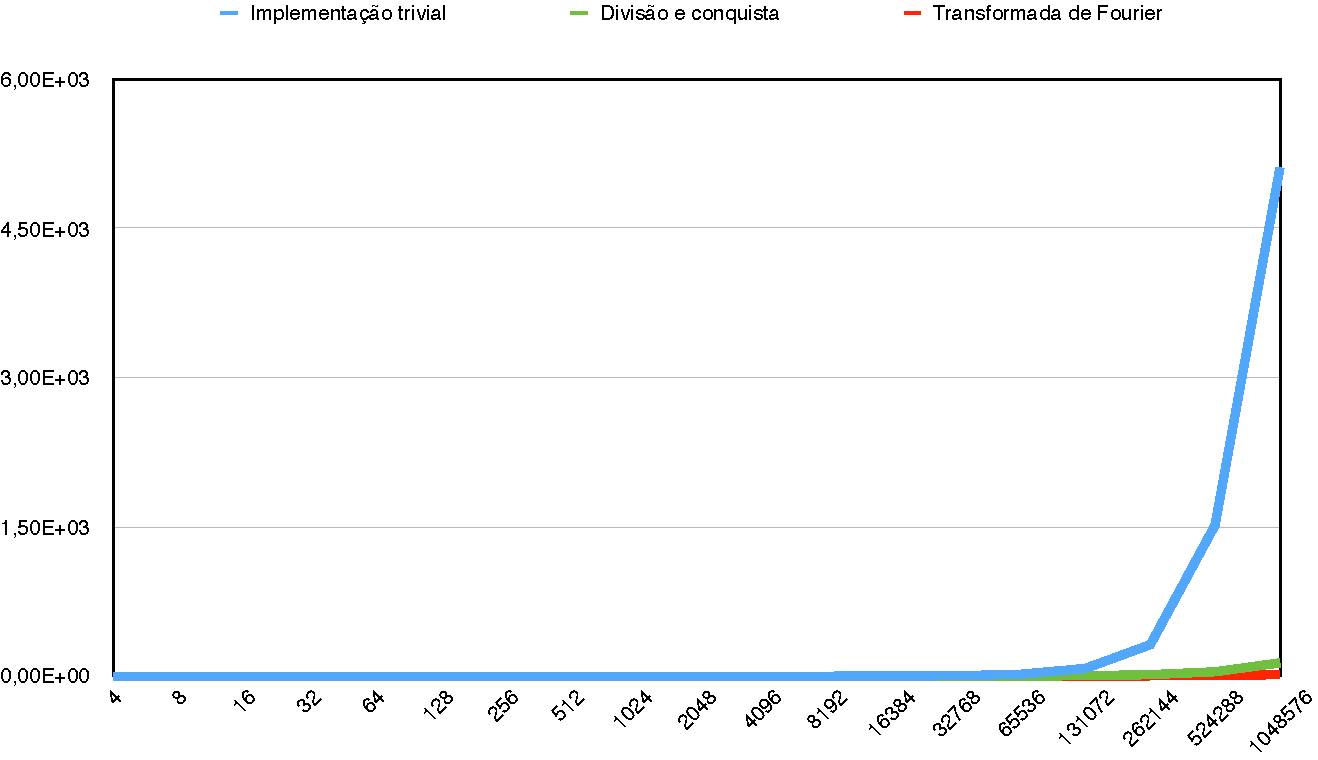
\includegraphics[width=6.4in]{charts/mult_time.pdf}
 \caption{Gráfico comparativo entre o TEMPO DE CPU dos algoritmos para o problema de multiplicação de polinômios.}
 \label{fig:AlutGraphTimeAll}
\end{figure}

\begin{figure}[H]
 \centering
 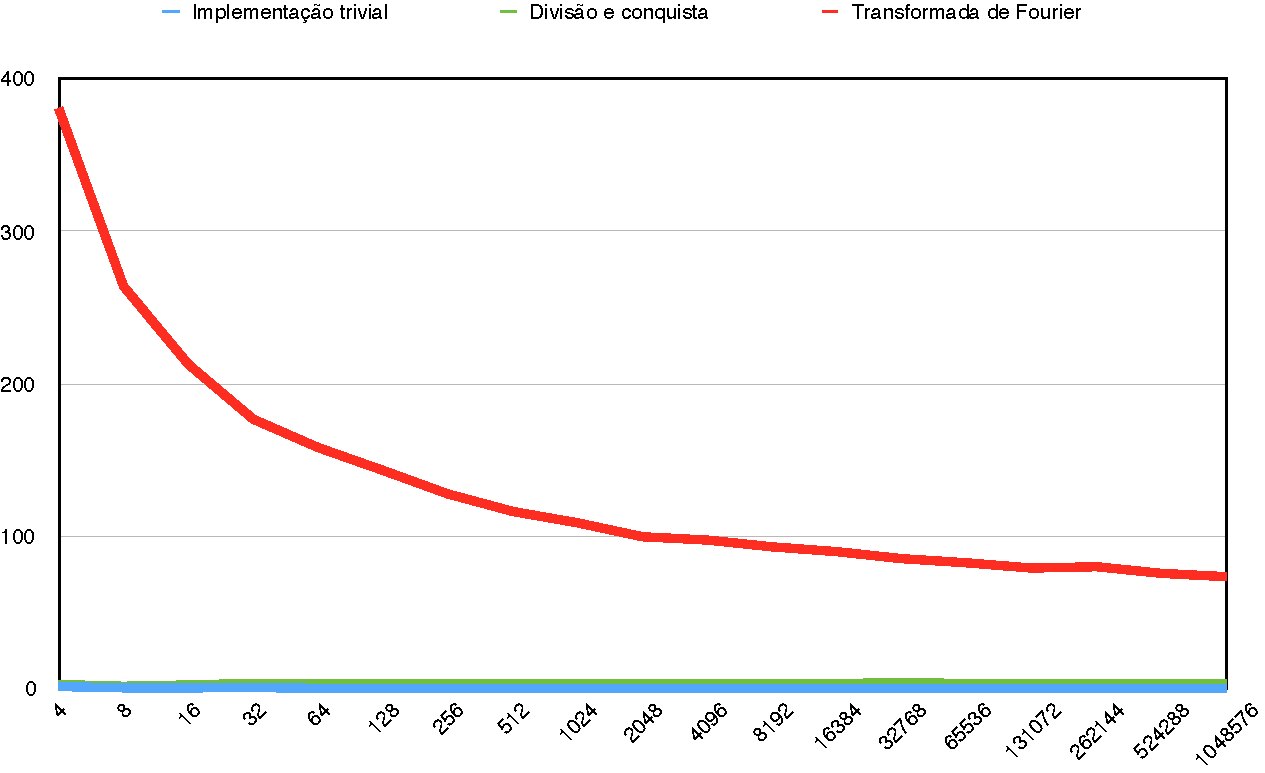
\includegraphics[width=6.4in]{charts/mult_raz.pdf}
 \caption{Gráfico comparativo entre as RAZÕES dos algoritmos para o problema de multiplicação de polinômios.}
 \label{fig:AlutGraphTimeAll}
\end{figure}


% ---
% Finaliza a parte no bookmark do PDF, para que se inicie o bookmark na raiz
% ---
\bookmarksetup{startatroot}% 
% ---

% ---
% Conclusão
% ---
\chapter*[Conclusão]{Conclusão}
\addcontentsline{toc}{chapter}{Conclusão}

No problema da mochila fracionaria o trabalho mostra que os algoritmos comportaram-se da seguinte forma:

\begin{center}
\textbf{Mediana das Medianas < Heapsort < Pivô}
\end{center}
Apesar da complexidade teórica do algoritmo Mediana das Medianas ser $O(n)$, o algoritmo do Pivô obteve melhor desempenho para instâncias executados. Tal fato ocorreu porque a Mediana das Medianas executou um número operações maior que número de operações para calcular o Pivô. Contudo, conforme apresentado na sessão 1.3, no pior caso o algoritmo do Pivô tem uma complexidade de $O(n\textsuperscript{2})$.

No problema de multiplicação de polinômios, os resultados mostram que, para um número grande de coeficientes ($n > 4096$), os algoritmos comportam-se da seguinte forma:
\begin{center}
\textbf{Transformada de Fourier < Karatsuba < Trivial}
\end{center}
Percebe-se que as razões entre a complexidade teórica e o tempo de execução mantiveram-se constante no Trivial e no Karatsuba. Apesar da Transformada de Fourier ter sido a mais rápida, as razões entre a complexidade teórica e o tempo de execução não se mantiveram constantes. Isso deve-se ao fato de que o algoritmo usado para execução da FFT é uma implementação amadora, inspirado no pseudo-código do \cite{cormen2009}, feita por terceiros. Não foi possível garantir que a complexidade na prática, dessa implementação, seja exatamente $O(n*log(n))$. Uma possível solução para esse problema seria usar o pacote \cite{fftw} que disponibiliza diversas implementações de transformada de Fourier em linguagem C, e garante a complexidade teórica na prática.

É interessante notar que a implementação Trivial tem um ótimo tempo de execução para valores de $n < 4096$. Uma possível explicação é que os algoritmos de Karatsuba e de FFT utilizados fazem muita alocação dinâmica e chamadas recursivas. Quando n é pequeno, essa quantidade de alocações dinâmicas e chamadas recursivas prejudicam o tempo de execução mais do que o tamanho de n. Nestes casos, a multiplicação trivial mostrou-se mais interessante por sua simplicidade. Deve-se lembrar que o caso base do Karatsuba, mostrado na listagem \ref{divisao_conquista}, é uma execução do Trivial. Portanto, com poucos coeficientes, faz sentido o tempo de execução ser bem próximo.

Os códigos utilizados no desenvolvimento deste projeto podem ser integralmente acessados no repositório do Github.~\footnote{https://github.com/Busson/puc-rio.paa-2017.1-poggi}





















% ----------------------------------------------------------
% Referências bibliográficas
% ----------------------------------------------------------
\bibliography{abntex2-modelo-references}


% ----------------------------------------------------------
% Apêndices
% ----------------------------------------------------------
% Inicia os apêndices
% ---
% \begin{apendicesenv}

% \chapter{Lorem Ipsum}

% \end{apendicesenv}


% ----------------------------------------------------------
% Anexos
% ----------------------------------------------------------
% % Inicia os anexos
% ---
% \begin{anexosenv}

% \chapter{Lorem Ipsum}

% \end{anexosenv}


\printindex

\end{document}


% Este documento e seu código-fonte são exemplos de referência de uso da classe
% \textsf{abntex2} e do pacote \textsf{abntex2cite}. O documento 
% exemplifica a elaboração de relatórios técnicos e/ou científicos produzidos
% conforme a ABNT NBR 10719:2011 \emph{Informação e documentação - Relatório
% técnico e/ou científico - Apresentação}.

% A expressão ``Modelo canônico'' é utilizada para indicar que \abnTeX\ não é
% modelo específico de nenhuma universidade ou instituição, mas que implementa tão
% somente os requisitos das normas da ABNT. Uma lista completa das normas
% observadas pelo \abnTeX\ é apresentada em \citeonline{abntex2classe}.

% Sinta-se convidado a participar do projeto \abnTeX! Acesse o site do projeto em
% \url{http://abntex2.googlecode.com/}. Também fique livre para conhecer,
% estudar, alterar e redistribuir o trabalho do \abnTeX, desde que os arquivos
% modificados tenham seus nomes alterados e que os créditos sejam dados aos
% autores originais, nos termos da ``The \LaTeX\ Project Public
% License''\footnote{\url{http://www.latex-project.org/lppl.txt}}.

% Encorajamos que sejam realizadas customizações específicas deste exemplo para
% universidades e outras instituições --- como capas, folhas de rosto, etc.
% Porém, recomendamos que ao invés de se alterar diretamente os arquivos do
% \abnTeX, distribua-se arquivos com as respectivas customizações.
% Isso permite que futuras versões do \abnTeX~não se tornem automaticamente
% incompatíveis com as customizações promovidas. Consulte
% \citeonline{abntex2-wiki-como-customizar} par mais informações.

% Este documento deve ser utilizado como complemento dos manuais do \abnTeX\ 
% \cite{abntex2classe,abntex2cite,abntex2cite-alf} e da classe \textsf{memoir}
% \cite{memoir}. 